% =============================================================================
% mcp-kicad-vscode — Artigo científico/tecnológico
% Autor: William da Silva Vianna — Instituto Federal Fluminense (IFF)
%
% Compilação: pdflatex -> bibtex -> pdflatex -> pdflatex
%   ./build.sh          (gera artigo-mcp-kicad-vscode.pdf)
%
% Alternativas de título avaliadas (mantido o primeiro):
%   1. mcp-kicad-vscode: automação do fluxo de projeto de placas de circuito
%      impresso no KiCad por meio do Model Context Protocol (ESCOLHIDO)
%   2. Um servidor Model Context Protocol para projeto assistido de PCBs no KiCad
%   3. Integração de assistentes de IA ao KiCad via Model Context Protocol:
%      arquitetura, implementação e estudo de caso
%   4. Conectando modelos de linguagem ao fluxo de projeto de PCBs: o servidor
%      mcp-kicad-vscode
% =============================================================================
\documentclass[11pt,a4paper]{article}

\usepackage[utf8]{inputenc}
\usepackage[T1]{fontenc}
\usepackage[brazil]{babel}
\shorthandoff{"}

\usepackage[margin=2.5cm]{geometry}
\usepackage{amsmath}
\usepackage{amssymb}
\usepackage{graphicx}
\graphicspath{{figures/}}
\usepackage{booktabs}
\usepackage{array}
\usepackage{float}
\usepackage{caption}
\usepackage{enumitem}
\usepackage{xcolor}
\usepackage{tikz}
\usetikzlibrary{arrows.meta,positioning,shapes.geometric,fit,backgrounds}
\usepackage[numbers]{natbib}
\usepackage[hidelinks]{hyperref}

% Palavras-chave e demais metadados -------------------------------------------------
\title{\textbf{mcp-kicad-vscode: automação do fluxo de projeto de placas de
circuito impresso no KiCad por meio do Model Context Protocol}}

\author{
  William da Silva Vianna\\
  \small Instituto Federal Fluminense (IFF)\\
  \small Campos dos Goytacazes, RJ, Brasil
}

\date{}

\begin{document}

\maketitle

\begin{abstract}
\noindent
A crescente adoção de assistentes baseados em grandes modelos de linguagem
(LLMs) na engenharia cria uma demanda por integrações padronizadas entre esses
assistentes e ferramentas de automação de projeto eletrônico (EDA). Este
trabalho analisa e avalia o \texttt{mcp-kicad-vscode}, um servidor
\emph{Model Context Protocol} (MCP) de código aberto (projeto
\texttt{KiCAD-MCP-Server}, de \emph{mixelpixx}) que expõe operações do KiCad
--- projeto, esquemático, layout de placa, roteamento, verificação de regras,
exportação de fabricação e integrações com catálogos de componentes --- a
assistentes de IA. O sistema adota arquitetura em duas camadas (TypeScript
para o protocolo MCP e
Python para a interface com o \emph{pcbnew}/IPC), registra 233 ferramentas
organizadas em 24 módulos funcionais, disponibiliza 173 delas para descoberta
por palavra-chave em 16 categorias e expõe 23 recursos dinâmicos de estado do
projeto. A validação combinou métricas de implementação, execução das suítes de
teste (84 casos TypeScript e 2.367 casos Python) e um estudo de caso, conduzido
pelo autor, com uma placa seguidora de linhas de quatro camadas
(97 \emph{footprints}, 83 redes, 82,1\,mm $\times$ 80,2\,mm). Os resultados
locais apontam 84/84 testes
TypeScript aprovados e 2.328/2.367 casos Python aprovados (8 falhas e 31
ignorados), além de verificação de regras de projeto que identificou 11
violações residuais (9 erros; 2 avisos) e zero itens não conectados. Discutem-se
limitações --- integração IPC não exercitada no ambiente de validação, 60
ferramentas ainda não indexadas e ausência de estudo com usuários --- e
trabalhos futuros.
\end{abstract}

\noindent\textbf{Palavras-chave:} Model Context Protocol; KiCad; projeto de
placas de circuito impresso; assistentes de IA; automação de EDA.

\section{Introdução}\label{sec:introducao}

O projeto de placas de circuito impresso (PCB, do inglês \emph{printed circuit
board}) é uma atividade multidisciplinar que combina decisões elétricas,
térmicas, mecânicas e de manufatura. Nas últimas décadas, o setor consolidou
fluxos de trabalho fortemente assistidos por computador, nos quais ferramentas
de automação de projeto eletrônico (EDA) executam desde a captura esquemática
até a geração de arquivos de fabricação, passando por verificação de regras de
projeto (DRC, \emph{design rule check}) e roteamento assistido
\citep{kicaddocs,horowitz2015}.

Paralelamente, assistentes de programação e engenharia baseados em grandes
modelos de linguagem (LLMs) passaram a atuar como agentes capazes de planejar e
executar ações em computadores, desde que recebam interfaces adequadas às suas
capacidades \citep{yao2023react,yang2024sweagent}. Quando o alvo é um
\emph{software} de engenharia desktop, como o KiCad, o obstáculo deixa de ser a
capacidade de raciocínio do modelo e passa a ser a ausência de uma camada de
integração padronizada, descobrível e verificável entre o assistente e as
operações da ferramenta.

Em novembro de 2024, a Anthropic publicou o \emph{Model Context Protocol} (MCP),
um protocolo aberto baseado em JSON-RPC 2.0 que padroniza a forma como
aplicações hospedeiras (\emph{hosts}) expõem \emph{tools}, \emph{resources} e
\emph{prompts} a modelos de linguagem \citep{anthropic2024mcp,mcp2025spec}. A
proposta reduz o custo de integração de $N \times M$ conectores proprietários
para um único protocolo, permitindo que um mesmo servidor seja utilizado por
diferentes clientes (editores de código, ambientes de chat e agentes
autônomos).

Este trabalho parte da seguinte questão de pesquisa: \emph{como expor de forma
ampla, descobrível e testável o fluxo de projeto de PCBs do KiCad a assistentes
de IA, preservando a robustez exigida por operações destrutivas sobre arquivos
de projeto?} Para respondê-la, foi especificado, implementado e avaliado o
\texttt{mcp-kicad-vscode}, um servidor MCP que traduz operações do KiCad em
ferramentas executáveis por agentes, com integração a catálogos reais de
componentes e a roteador automático.

As principais contribuições deste trabalho são:

\begin{enumerate}[leftmargin=1.4em,itemsep=0.25em]
  \item a especificação e implementação de uma arquitetura em duas camadas
        (TypeScript para o protocolo MCP; Python para a interface com a API
        \emph{pcbnew}/IPC do KiCad), com abstração de \emph{backends} e
        correlação de requisições entre os processos;
  \item um catálogo de 233 ferramentas MCP organizadas em 24 módulos
        funcionais, cobrindo esquemático, placa, roteamento, regras de
        projeto, exportação, bibliotecas, criação de partes, datasheets e
        cadeia de suprimentos;
  \item um mecanismo de descoberta por palavra-chave (\texttt{search\_tools},
        \texttt{get\_category\_tools}) que indexa 173 ferramentas em 16
        categorias, além de 23 recursos dinâmicos que expõem o estado do
        projeto;
  \item uma estratégia de qualidade que combina testes automatizados em duas
        linguagens (84 casos em TypeScript e 2.367 casos coletados em Python),
        integração contínua em múltiplos sistemas operacionais e geração
        automática do inventário de ferramentas;
  \item uma avaliação por estudo de caso com uma placa seguidora de linhas de
        quatro camadas projetada no workspace, incluindo verificação de regras
        por \texttt{kicad-cli}, quantificação de violações residuais e
        análise crítica das limitações.
\end{enumerate}

O restante do artigo está organizado da seguinte forma: a
Seção~\ref{sec:fundamentacao} apresenta a fundamentação teórica e os trabalhos
relacionados; a Seção~\ref{sec:metodologia} descreve os materiais e métodos,
incluindo a arquitetura do servidor e o desenho da avaliação; a
Seção~\ref{sec:resultados} reporta os resultados e a
Seção~\ref{sec:discussao} os discute; por fim, a
Seção~\ref{sec:conclusao} conclui o trabalho e aponta direções futuras.

\section{Fundamentação teórica e trabalhos relacionados}\label{sec:fundamentacao}

\subsection{O Model Context Protocol}

O MCP é um protocolo aberto que padroniza a comunicação entre aplicações de IA
e fontes externas de contexto e execução \citep{anthropic2024mcp}. Sua
especificação define uma arquitetura cliente--servidor na qual o
\emph{host} (por exemplo, um editor de código ou assistente conversacional)
instancia um cliente MCP por servidor conectado. A comunicação emprega
JSON-RPC 2.0 e pode ocorrer por entrada/saída padrão (\emph{stdio}) ou por
transportes HTTP com streaming \citep{mcp2025spec}.

O protocolo define três primitivas principais que um servidor pode oferecer
\citep{mcp2025docs}:

\begin{itemize}[leftmargin=1.4em,itemsep=0.2em]
  \item \textbf{Tools}: funções executáveis, descritas por esquema JSON, que o
        modelo pode invocar para produzir efeitos (criar arquivos, modificar
        geometria, executar verificações);
  \item \textbf{Resources}: dados somente leitura identificados por URI, como o
        estado de um projeto ou listas de componentes;
  \item \textbf{Prompts}: modelos de interação predefinidos que orientam o
        uso do servidor para tarefas recorrentes.
\end{itemize}

A especificação utilizada nesta implementação é a de 18 de junho de 2025
\citep{mcp2025spec}, que consolida o ciclo de vida de inicialização,
negociação de capacidades e transporte. A adoção do MCP por diferentes
fornecedores de modelos e editores reduziu o acoplamento entre assistentes e
ferramentas, tornando viável publicar um único servidor para todo um domínio,
como o projeto de PCBs.

\subsection{Agentes baseados em LLMs e uso de ferramentas}

A capacidade de um agente de interagir com o ambiente depende não apenas do
modelo, mas do desenho da interface que lhe é oferecida. \citet{yao2023react}
demonstram que intercalar raciocínio e ação melhora o desempenho em tarefas
que exigem decisões encadeadas. \citet{schick2023toolformer} e
\citet{patil2023gorilla} evidenciam que modelos podem aprender a invocar APIs
e ferramentas externas com acurácia crescente quando as chamadas são expostas
de forma estruturada. \citet{yang2024sweagent} mostram, no contexto de
engenharia de software, que a interface agente--computador (ACI) tem impacto
direto no desempenho: nomes de comandos claros, saídas concisas e
descobribilidade de ferramentas importam tanto quanto o modelo utilizado.

Esses resultados motivam decisões de projeto adotadas neste trabalho: exposição
individual de cada ferramenta (sem roteador oculto), descrições objetivas,
mecanismos explícitos de descoberta e respostas padronizadas e testáveis.

\subsection{Automação de EDA e o KiCad}

O KiCad é uma suíte de EDA de código aberto que abrange captura esquemática,
layout de placa, bibliotecas de símbolos e \emph{footprints}, visualização 3D e
geração de arquivos de fabricação \citep{kicaddocs}. Seus arquivos de projeto
são expressões-S (\emph{S-expressions}) versionáveis em texto, o que facilita
automação e revisão por ferramentas externas.

A extensibilidade do KiCad se apoia em três mecanismos complementares:
(i) a API Python \texttt{pcbnew}, disponibilizada por meio de \emph{bindings}
SWIG \citep{swig}; (ii) a API IPC, que permite comunicação em tempo real com a
interface gráfica; e (iii) o utilitário de linha de comando \texttt{kicad-cli},
que executa exportações e verificações de forma independente da interface
gráfica \citep{kicadcli,kicaddev}. Esses mecanismos são a base de integrações
automatizadas, inclusive as conduzidas por agentes de IA.

\subsection{Trabalhos relacionados}

A aplicação de LLMs ao domínio de \emph{design} de circuitos tem exemplos
relevantes. \citet{liu2023chipnemo} adaptam modelos ao domínio de projeto de
\emph{chips} industriais (assistente de engenharia, geração de \emph{scripts}
de EDA e análise de defeitos), demonstrando ganhos com especialização de
domínio. Trabalhos dessa natureza, no entanto, concentram-se na adaptação do
\emph{modelo} a um domínio; a integração entre assistentes genéricos e
ferramentas de EDA permanece fragmentada, tipicamente resolvida por
\emph{scripts} específicos e não reutilizáveis.

Do lado das ferramentas, a automação do KiCad por \emph{scripts} Python é
consolidada, porém cada integração reproduz decisões de sessão, tratamento de
erros e descoberta de operações. O MCP altera esse cenário ao oferecer um
contrato único entre assistentes e ferramentas \citep{mcp2025spec}. Neste
contexto, o \texttt{mcp-kicad-vscode} se posiciona como um servidor MCP de
propósito geral para o fluxo de PCB no KiCad, com cobertura ampla,
integrações de fabricação e suíte de testes própria --- combinação ainda
escassa na literatura e no ecossistema de código aberto.

A lacuna endereçada é, portanto, dupla: (i) ausência de uma camada padronizada
e descobrível que cubra o ciclo de projeto de PCB de ponta a ponta
(esquemático, layout, verificação, fabricação); e (ii) ausência de evidências
publicadas sobre robustez e manutenibilidade desse tipo de integração,
incluindo o comportamento sob operações destrutivas e a cobertura de testes.

\section{Materiais e métodos}\label{sec:metodologia}

\subsection{Delineamento da pesquisa}

Este trabalho caracteriza-se como pesquisa aplicada de natureza tecnológica,
conduzida por meio de desenvolvimento de sistema e avaliação por estudo de caso
instrumental. O percurso metodológico compreendeu cinco etapas:
(i) auditoria do domínio e do código-fonte do servidor;
(ii) definição de requisitos do sistema e da API MCP exposta;
(iii) implementação e evolução da arquitetura em duas camadas;
(iv) verificação automatizada por suítes de teste e integração contínua;
(v) estudo de caso com uma placa de quatro camadas projetada no mesmo
\emph{workspace}.

Não se trata de experimento controlado com grupo de comparação: a avaliação
adota métricas descritivas de implementação (contagem de ferramentas, recursos,
linhas de código e casos de teste), resultados de execução das suítes e
indicadores de verificação de projeto (regras do KiCad) obtidos sobre um
artefato real. As ameaças à validade dessa escolha são discutidas na
Seção~\ref{sec:discussao}.

\subsection{Requisitos do sistema}

Os requisitos que orientaram a implementação estão sintetizados na
Tabela~\ref{tab:requisitos}, com a forma de atendimento e a evidência
correspondente.

\begin{table}[htbp]
\centering
\small
\caption{Requisitos do servidor e evidências de atendimento.}
\label{tab:requisitos}
\begin{tabular}{@{}p{0.8cm}p{4.0cm}p{5.4cm}p{4.2cm}@{}}
\toprule
\textbf{ID} & \textbf{Requisito} & \textbf{Implementação} & \textbf{Evidência} \\
\midrule
R1 & Cobrir o fluxo de PCB de ponta a ponta & 233 ferramentas em 24 módulos (projeto, esquemático, roteamento, regras, exportação) & Inventário gerado (\texttt{docs/TOOL\_INVENTORY.md}) e Seção~\ref{sec:resultados} \\
R2 & Permitir descoberta de operações pelo agente & Registro com categorias, lista de essenciais e \texttt{search\_tools} / \texttt{get\_category\_tools} & 173 ferramentas indexadas em 16 categorias \\
R3 & Ser robusto sob falhas e respostas fora de ordem & Correlação de requisições com identificadores, descarte de respostas tardias, tempos-limite por comando & Testes de correlação e de \emph{startup} em \texttt{tests-ts/} \\
R4 & Preservar integridade dos arquivos do usuário & \emph{Saves} explícitos, sessão fixada por \emph{backend}, validação prévia de esquemáticos corrompidos & Suíte Python (\texttt{tests/}) e histórico de correções do projeto \\
R5 & Ser portável (Linux, Windows, macOS) & Node.js + Python portáveis; \emph{launcher} com variáveis específicas por plataforma & Matriz de CI em quatro sistemas operacionais \\
R6 & Ser verificável e extensível & Testes em duas linguagens, inventário gerado automaticamente como \emph{gate} de CI & 84 casos TypeScript e 2.367 casos Python; verificação \texttt{docs:tools:check} \\
\bottomrule
\end{tabular}
\end{table}

\subsection{Arquitetura do servidor}\label{subsec:arquitetura}

O sistema adota arquitetura em duas camadas, ilustrada na
Figura~\ref{fig:arquitetura}. A camada externa implementa o protocolo MCP em
TypeScript, registra as ferramentas com esquemas de validação e gerencia o
ciclo de vida do processo Python. A camada interna, em Python, traduz comandos
em operações do KiCad por meio de dois \emph{backends} intercambiáveis:
a API \texttt{pcbnew} (SWIG) e a API IPC \citep{kicadcli,kicaddev,swig}. A
seleção do \emph{backend} é automática, com queda para SWIG quando a API IPC
não está disponível.

\begin{figure}[htbp]
\centering
\begin{tikzpicture}[
  font=\footnotesize,
  box/.style={draw, rounded corners=2pt, align=center, inner sep=4pt},
  arr/.style={-{Stealth[length=2mm]}, thick},
  trace/.style={-{Stealth[length=2mm]}, thick, dashed},
  node distance=6mm and 8mm
]
\node[box, fill=blue!6] (host) {Assistente de IA\\(host MCP)};
\node[box, fill=blue!12, right=of host] (ts) {Servidor MCP (TypeScript)\\233 ferramentas -- 16 categorias\\23 recursos --- esquemas};
\node[box, fill=orange!10, right=of ts] (py) {Interface Python\\\texttt{kicad\_interface.py}\\roteador de comandos};
\node[box, fill=green!10, right=of py] (kicad) {KiCad 9\\arquivos \texttt{.kicad\_pcb}\\\texttt{.kicad\_sch}};
\node[box, fill=gray!10, below=8mm of py] (cli) {\texttt{kicad-cli}\\(DRC, ERC, exportações)};
\node[box, fill=gray!10, above=8mm of py] (ipc) {API IPC\\(experimental)};
\draw[arr] (host) -- node[above, font=\scriptsize]{MCP (JSON-RPC 2.0)} (ts);
\draw[arr] (ts) -- node[above, font=\scriptsize]{JSON (NDJSON) + IDs} (py);
\draw[arr] (py) -- node[above, font=\scriptsize]{pcbnew (SWIG)} (kicad);
\draw[trace] (py) -- (ipc);
\draw[trace] (ipc) -- (kicad);
\draw[arr] (py) -- (cli);
\draw[arr] (cli) |- (kicad);
\end{tikzpicture}
\caption{Arquitetura em duas camadas do \texttt{mcp-kicad-vscode}. A camada
TypeScript fala MCP com o assistente; a camada Python opera o KiCad por SWIG,
IPC (experimental) ou \texttt{kicad-cli}.}
\label{fig:arquitetura}
\end{figure}

Cada ferramenta é registrada individualmente com \texttt{server.tool()}, isto é,
sem roteador que oculte esquemas do cliente MCP. O registro de categorias
existe para apoiar a \emph{descoberta} --- decisão alinhada à literatura sobre
interfaces agente--computador \citep{yang2024sweagent}: o agente pode tanto
chamar uma ferramenta conhecida quanto localizá-la por palavra-chave.

O protocolo interno entre as camadas usa JSON delimitado por linhas
(\emph{newline-delimited JSON}) com identificadores de requisição. Cada
resposta ecoa o identificador correspondente; respostas tardias de uma
requisição expirada são descartadas, evitando o desalinhamento entre pedido e
resposta que pode ocorrer após um tempo-limite. O processo Python é único e
persistente, iniciado na primeira chamada de ferramenta, e mantém o estado do
projeto em memória quando o \emph{backend} permite.

\subsection{Estratégia de qualidade}

A verificação adota três mecanismos complementares: (i) suítes de teste em
TypeScript (Vitest~\citep{vitest}) e Python (pytest~\citep{pytest}), incluindo
testes de correlação de requisições, completude do registro de ferramentas e
validação sintática; (ii) integração contínua~\citep{githubactions} com matriz
de sistemas operacionais e versões de \emph{runtime}; e (iii) geração
automática do inventário de ferramentas a partir do código, exigida como
condição de aceitação no CI (\texttt{npm run docs:tools:check}), impedindo que a
documentação diverga da implementação.

\subsection{Ambiente de validação}

A execução local ocorreu em estação de trabalho com Ubuntu 24.04.4 LTS
(\emph{kernel} 7.0.0-31), com KiCad 9.0.7 (pacote \emph{snap}, revisão 22),
Node.js~v22.23.2~\citep{nodejs}, npm~12.0.2, Python~3.12.3~\citep{python}
(ambiente virtual com as dependências de produção e de teste declaradas pelo
projeto) e pytest 9.1.1.
O utilitário \texttt{kicad-cli} 9.0.7 foi utilizado para verificação e
exportações fora da interface gráfica \citep{kicadcli}.

\subsection{Estudo de caso}

O estudo de caso utiliza a placa \texttt{seguidor\_de\_linhas\_4camada2-2026-1},
um projeto de quatro camadas para um robô seguidor de linhas, contendo
subsistemas de sensoriamento óptico reflexivo, conversão de energia
(\emph{MPPT}), acionamento de motores em ponte H, interface USB-C, regulação
de tensão e sinalização. O projeto foi analisado por meio de:
(i) contagem de \emph{footprints}, redes e folhas do esquemático;
(ii) execução de DRC com \texttt{kicad-cli pcb drc --format json
--severity-all};
(iii) renderizações 3D das faces superior e inferior; e
(iv) inspeção dos artefatos de fabricação gerados pelo fluxo de projeto.
Os comandos exatos e os artefatos resultantes estão preservados no repositório
do projeto (material suplementar digital), em especial no diretório
\texttt{evidencias/}.

\section{Resultados}\label{sec:resultados}

\subsection{Métricas de implementação e catálogo de ferramentas}

A implementação reúne 42 arquivos TypeScript (14.677 linhas) na camada MCP e
54.442 linhas em Python na camada de interface, das quais 38.050 no módulo de
comandos e 6.529 no roteador principal (\texttt{kicad\_interface.py}). O
servidor registra \textbf{233 ferramentas}, organizadas em 24 módulos
funcionais, agrupadas na Tabela~\ref{tab:categorias} em dez macro-áreas.

\begin{table}[htbp]
\centering
\small
\caption{Ferramentas MCP por macro-área funcional.}
\label{tab:categorias}
\begin{tabular}{@{}p{5.6cm}p{1.6cm}p{7.2cm}@{}}
\toprule
\textbf{Macro-área} & \textbf{N.\ de ferramentas} & \textbf{Módulos de origem} \\
\midrule
Esquemático (autoria, lote, hierarquia, acabamento) & 65 & \texttt{schematic.ts}, \texttt{schematic-batch.ts}, \texttt{schematic-hierarchy.ts}, \texttt{schematic-layout.ts} \\
Bibliotecas e criação de partes & 31 & \texttt{library.ts}, \texttt{library-symbol.ts}, \texttt{footprint.ts}, \texttt{symbol-creator.ts} \\
Projeto e ciclo de vida da placa & 31 & \texttt{project.ts}, \texttt{board.ts} \\
Componentes & 28 & \texttt{component.ts} \\
Exportação e fabricação & 27 & \texttt{export.ts} \\
Roteamento e autorouter & 21 & \texttt{routing.ts}, \texttt{freerouting.ts} \\
Datasheets e cadeia de suprimentos & 13 & \texttt{datasheet.ts}, \texttt{jlcpcb-api.ts}, \texttt{parts-registry.ts}, \texttt{digikey-api.ts} \\
Regras de projeto e validação & 9 & \texttt{design-rules.ts}, \texttt{validation.ts} \\
Interface do KiCad e descoberta & 6 & \texttt{ui.ts}, \texttt{router.ts} \\
Importação de formatos legados & 2 & \texttt{eagle.ts}, \texttt{pcb-import.ts} \\
\midrule
\textbf{Total} & \textbf{233} & 24 módulos \\
\bottomrule
\end{tabular}
\end{table}

Do total, 173 ferramentas (74,2\,\%) estão indexadas para descoberta por
palavra-chave em 16 categorias, conforme a Equação~\ref{eq:cobertura}; as 60
restantes permanecem executáveis, porém não localizáveis pelos mecanismos de
busca --- número que um teste automatizado congela para que só possa diminuir.
Além das ferramentas, o servidor expõe 23 recursos dinâmicos com o estado do
projeto (placa aberta, componentes, bibliotecas e informações do projeto) e
modelos de \emph{prompt} para tarefas recorrentes de projeto.

\begin{equation}
\label{eq:cobertura}
C_{desc} = \frac{173}{233} \approx 74{,}2\,\%.
\end{equation}

\subsection{Execução das suítes de teste}

A Tabela~\ref{tab:testes} consolida a execução local de 10 de setembro de 2026.
No total, 2.451 casos foram coletados; 2.412 foram aprovados (98,4\,\%), com 8
falhas e 31 casos ignorados. A suíte TypeScript passou integralmente
(84 de 84).

\begin{table}[htbp]
\centering
\small
\caption{Resultados da execução local das suítes de teste (10/09/2026).}
\label{tab:testes}
\begin{tabular}{@{}p{4.0cm}rrrrp{2.4cm}@{}}
\toprule
\textbf{Suíte} & \textbf{Casos} & \textbf{Aprov.} & \textbf{Falhas} & \textbf{Ignor.} & \textbf{Tempo} \\
\midrule
TypeScript (Vitest 2.1) & 84 & 84 & 0 & 0 & 1,5\,s \\
Python (pytest 9.1) & 2.367 & 2.328 & 8 & 31 & 45,0\,s \\
\midrule
\textbf{Total} & \textbf{2.451} & \textbf{2.412} & \textbf{8} & \textbf{31} & 46,5\,s \\
\bottomrule
\end{tabular}
\end{table}

As oito falhas concentram-se em casos que invocam o utilitário
\texttt{kicad-cli} como processo externo (importação Eagle, exportação de
netlist, verificação ERC e compatibilidade de formato de esquemático) e em um
teste de estado de módulo legado. A análise dos rastros de execução indica
sensibilidade ao ambiente de validação --- instalação do KiCad por pacote
\emph{snap}, sem o diretório \texttt{/usr/share/kicad/schemas} esperado por
alguns utilitários --- e não a regressões funcionais nas ferramentas exercitadas
pelos demais 2.328 casos aprovados. Os registros completos das execuções estão
preservados no repositório (\texttt{evidencias/}).

Em integração contínua, o projeto executa a suíte TypeScript em quatro
sistemas operacionais (Ubuntu 24.04, Ubuntu 22.04, Windows e macOS) com Node.js
20 e 22, a suíte Python em Ubuntu com Python 3.9 a 3.12, e dois portões de
qualidade adicionais: o \emph{lint} TypeScript e a verificação de que o
inventário de ferramentas está em dia com o código.

\subsection{Estudo de caso: placa seguidora de linhas de quatro camadas}

O projeto analisado possui 97 \emph{footprints} distribuídos em quatro camadas
de cobre (F.Cu, In1.Cu, In2.Cu e B.Cu), espessura total de 1,6\,mm e contorno
de aproximadamente 82,1\,mm $\times$ 80,2\,mm. O esquemático é hierárquico,
com nove folhas (raiz, fonte regulada, \emph{MPPT}, pontes H, sensores ópticos
reflexivos, interface USB-C e demais blocos), e a lista de materiais agrupa 37
itens. As Figura~\ref{fig:render-topo} e~\ref{fig:render-fundo} mostram
renderizações 3D geradas a partir do arquivo de placa; a
Figura~\ref{fig:esquematico} apresenta a folha raiz do esquemático, cujo bloco
de título registra a autoria do projeto.

\begin{figure}[htbp]
\centering
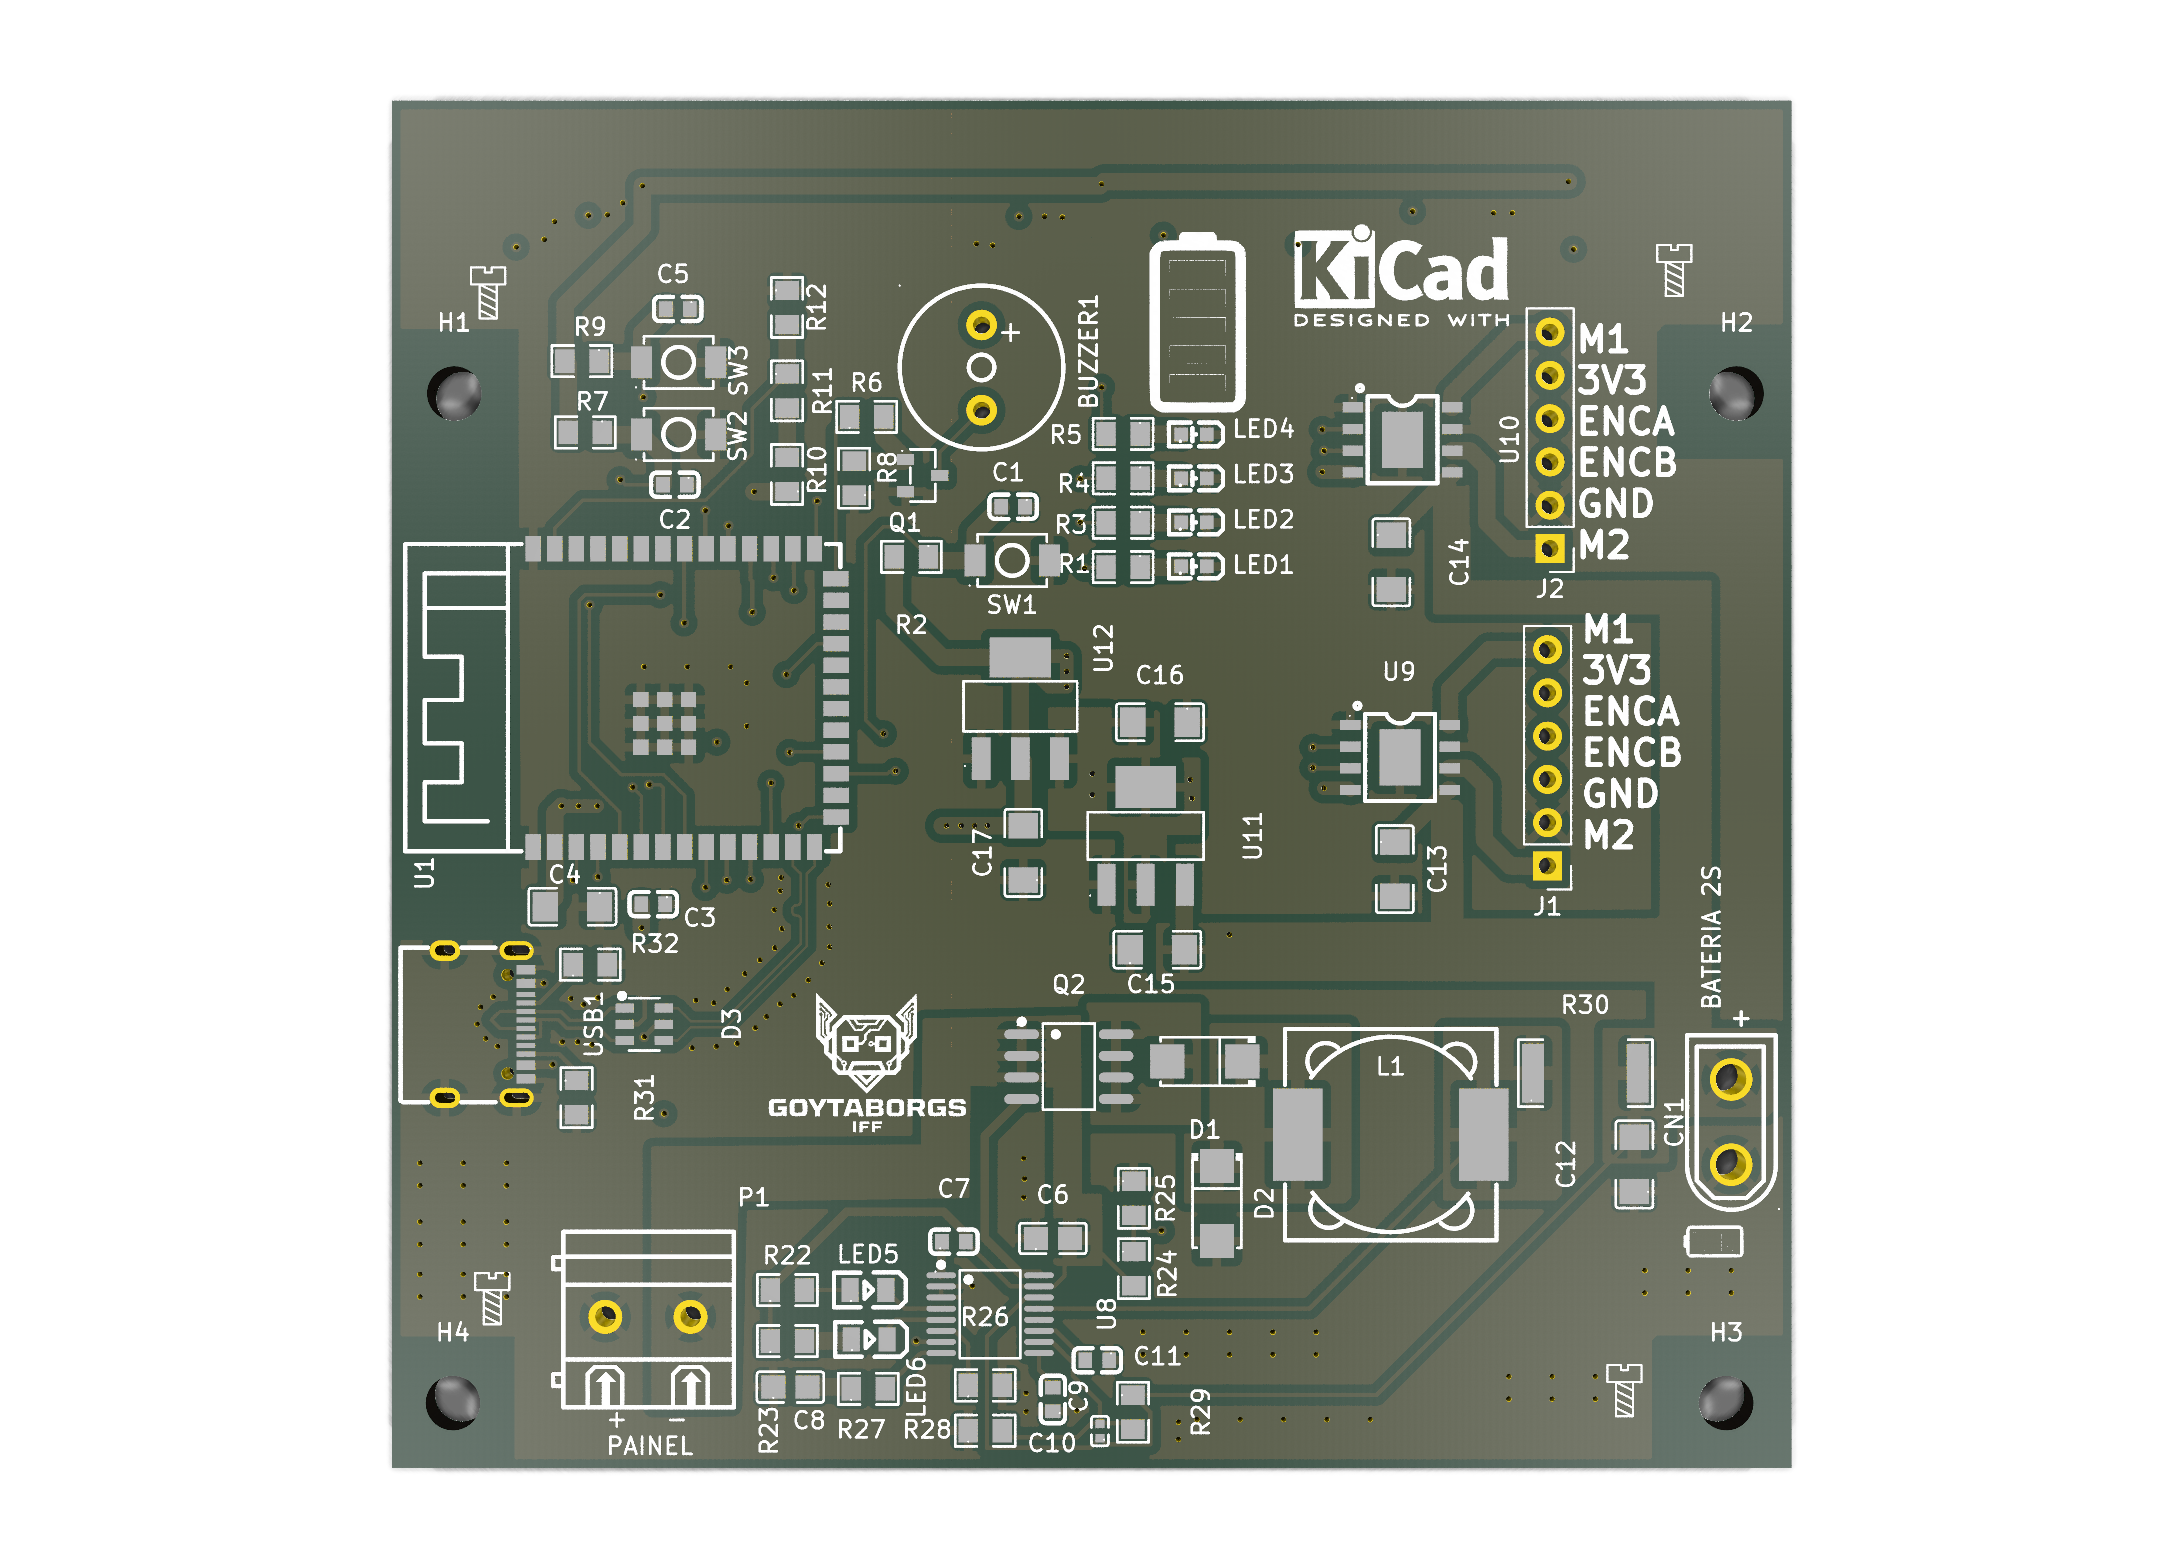
\includegraphics[width=0.82\textwidth]{pcb-render-topo.png}
\caption{Vista superior da placa seguidora de linhas (renderização 3D gerada
com \texttt{kicad-cli pcb render}).}
\label{fig:render-topo}
\end{figure}

\begin{figure}[htbp]
\centering
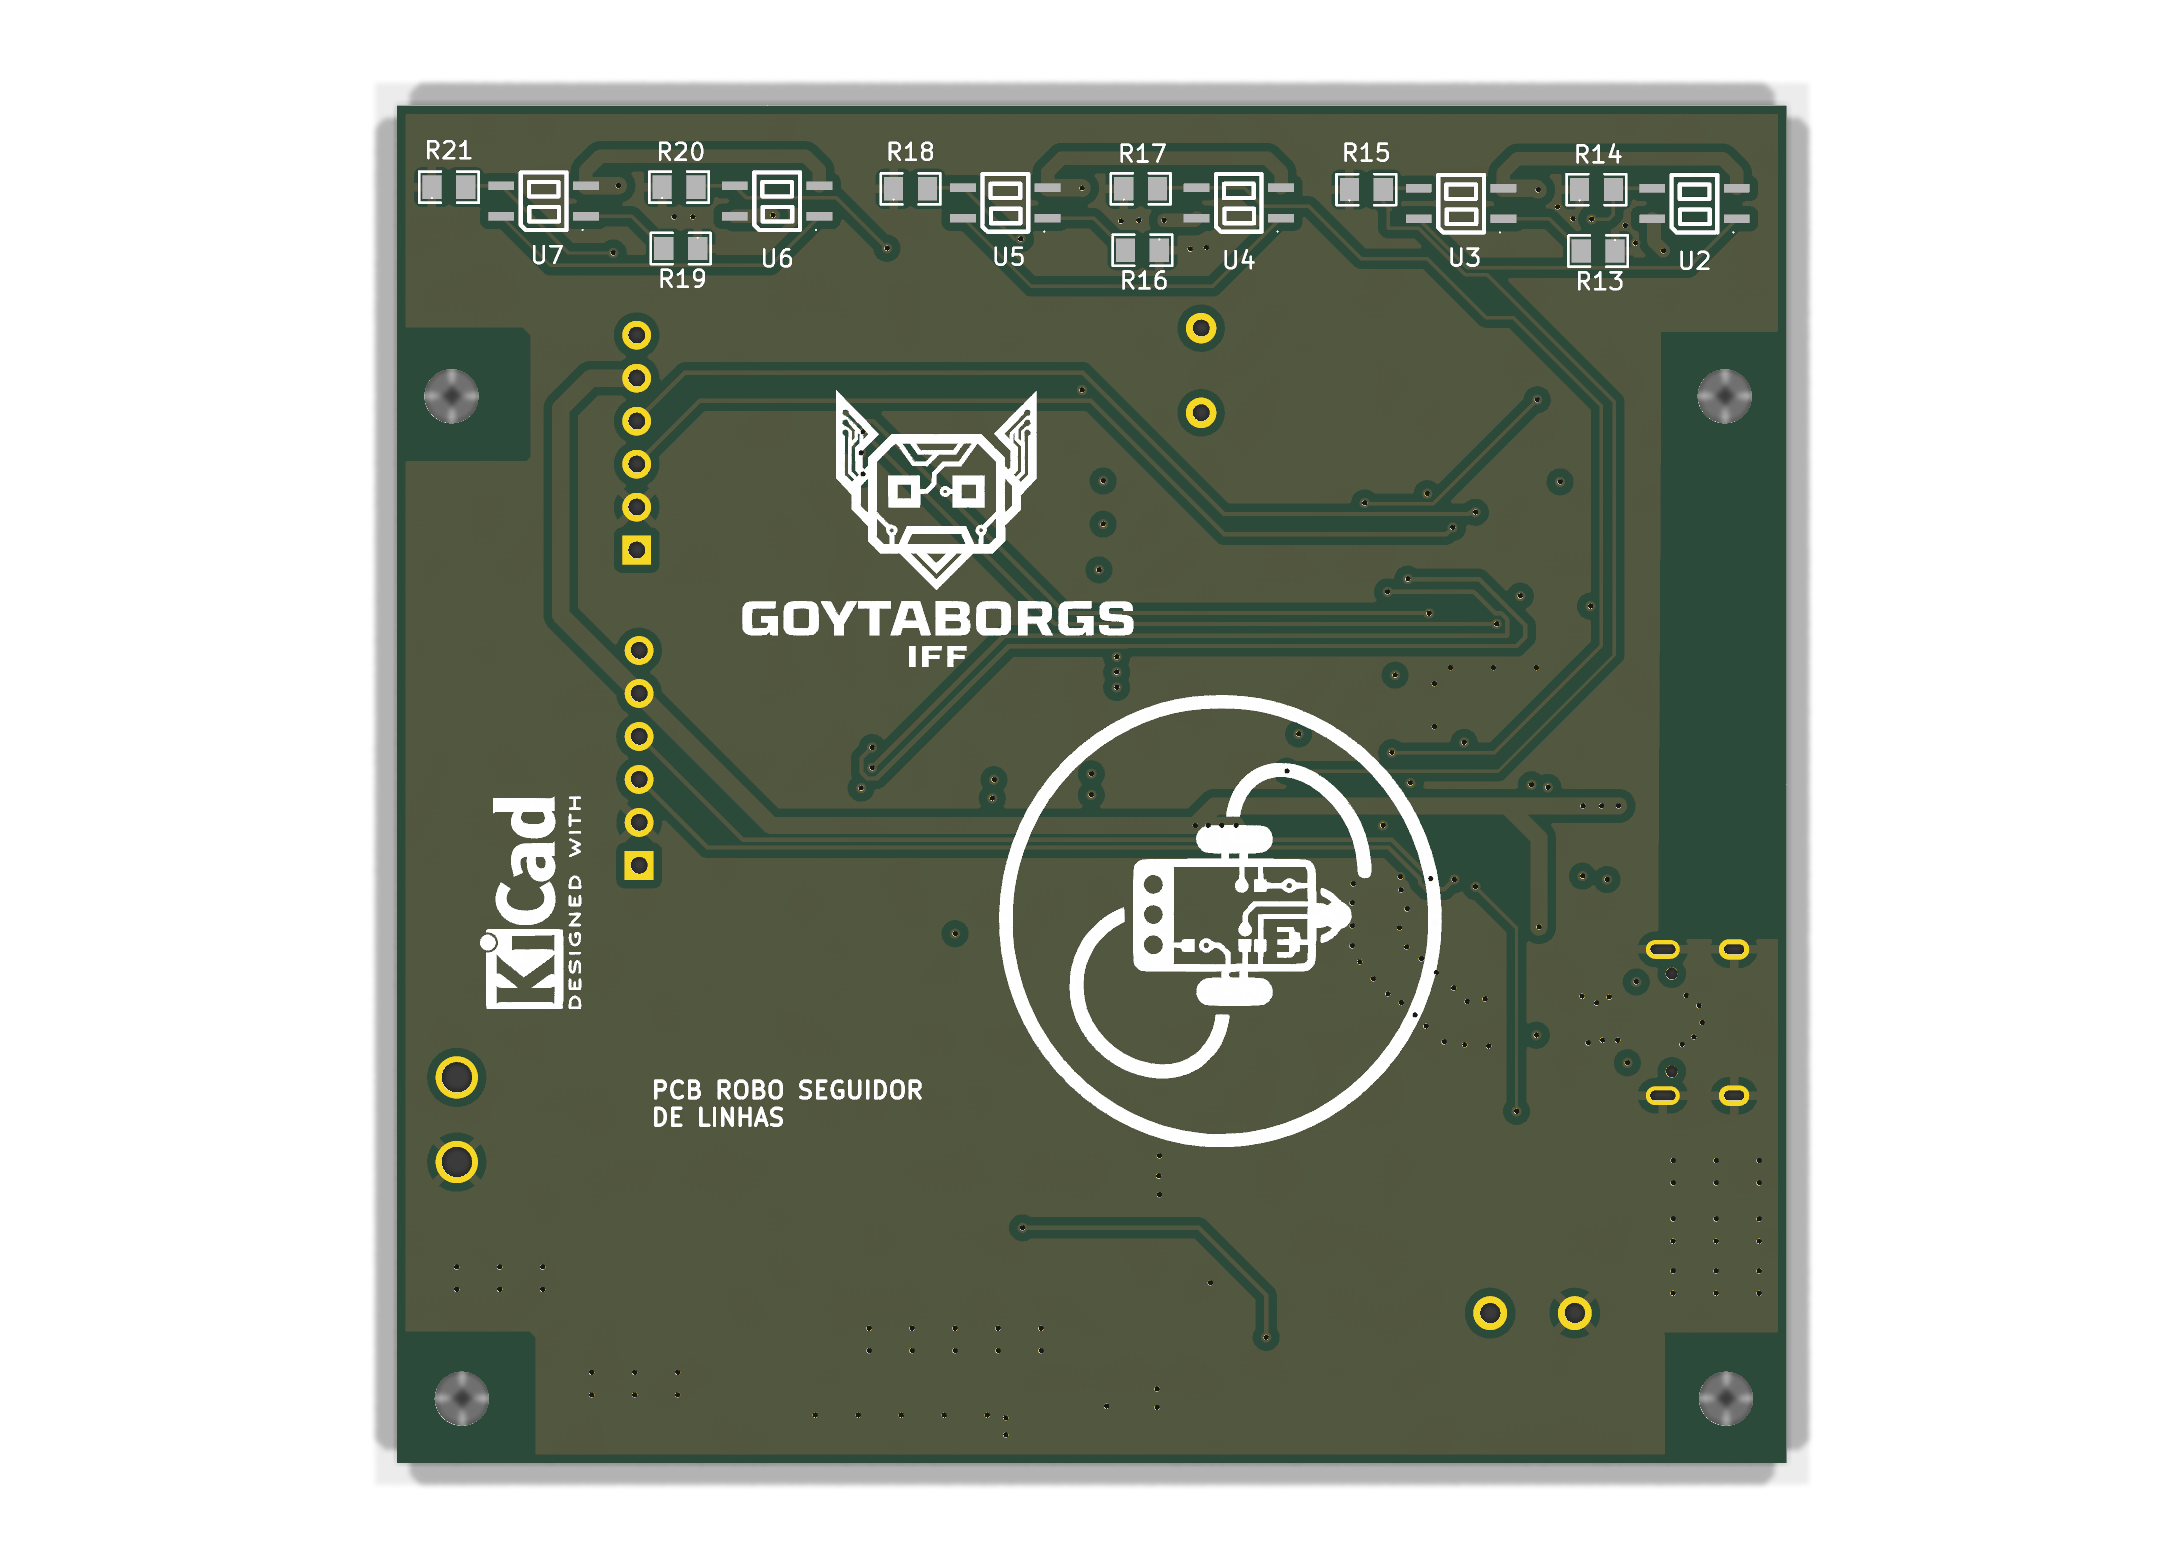
\includegraphics[width=0.82\textwidth]{pcb-render-fundo.png}
\caption{Vista inferior da placa, evidenciando o plano de cobre e a
distribuição dos componentes SMD.}
\label{fig:render-fundo}
\end{figure}

\begin{figure}[htbp]
\centering
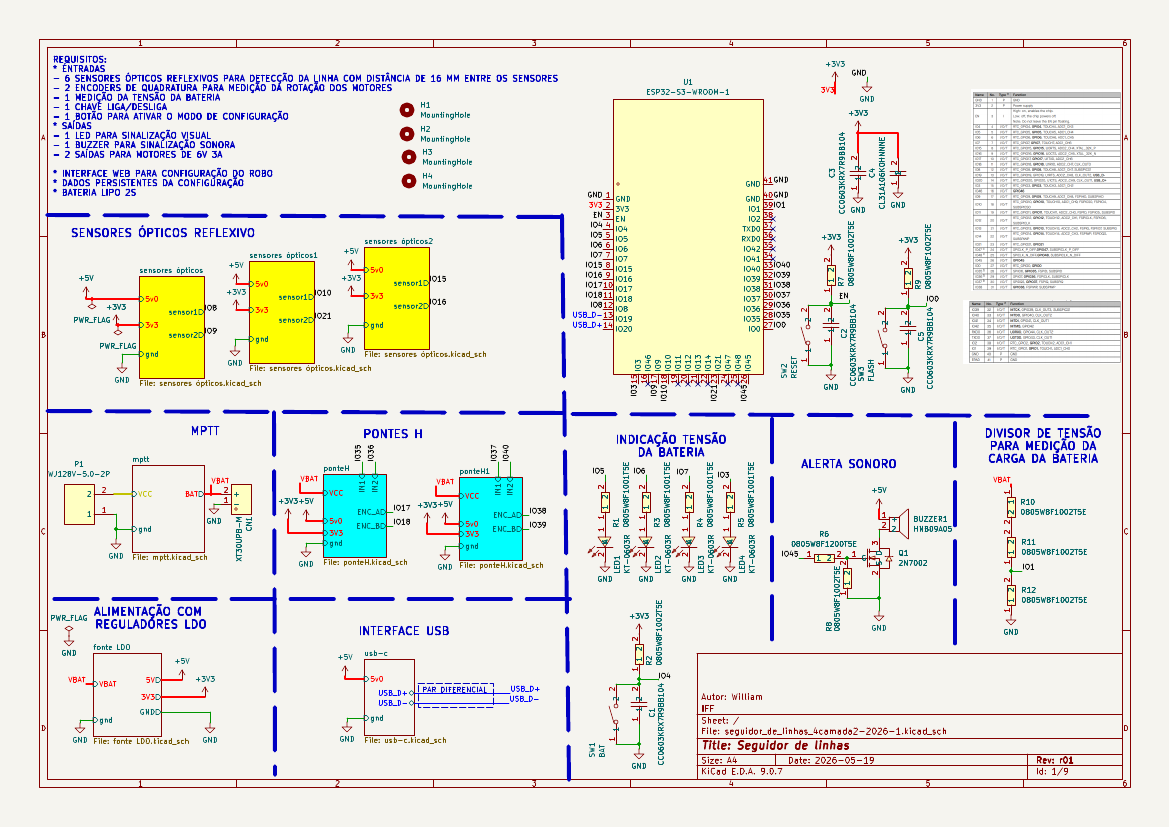
\includegraphics[width=0.95\textwidth]{esquematico-raiz.png}
\caption{Folha raiz do esquemático hierárquico (nove folhas), exportada com
\texttt{kicad-cli sch export pdf}.}
\label{fig:esquematico}
\end{figure}

A verificação de regras de projeto com \texttt{kicad-cli} 9.0.7 reportou
11 violações: 9 erros e 2 avisos, detalhados na
Tabela~\ref{tab:drc}. Não foram encontrados itens não conectados
(\emph{unconnected items}) nem divergências de paridade entre placa e
esquemático.

\begin{table}[htbp]
\centering
\small
\caption{Violações de DRC reportadas por \texttt{kicad-cli} 9.0.7 em 10/09/2026.}
\label{tab:drc}
\begin{tabular}{@{}p{3.4cm}p{1.9cm}p{1.2cm}p{8.0cm}@{}}
\toprule
\textbf{Tipo} & \textbf{Severidade} & \textbf{Qtde.} & \textbf{Diagnóstico} \\
\midrule
\texttt{annular\_width} & erro & 2 & Largura anular abaixo do mínimo de 0,100\,mm (medição de $-0{,}003$\,mm). \\
\texttt{clearance} & erro & 2 & Afastamento de 0,1812\,mm contra 0,200\,mm da classe \emph{Default}. \\
\texttt{malformed\_courtyard} & erro & 1 & \emph{Footprint} com \emph{courtyard} autointersectante. \\
\texttt{starved\_thermal} & erro & 4 & Conexão térmica à zona incompleta (1 de 2 raios exigidos). \\
\texttt{padstack} & aviso & 2 & \emph{Padstack} questionável (furo PTH sem cobre remanescente). \\
\bottomrule
\end{tabular}
\end{table}

O fluxo de projeto também produziu artefatos de fabricação no diretório
\texttt{production/} (lista de materiais, designadores, netlist IPC, arquivo de
posições e pacote compactado da placa), demonstrando a integração entre a
edição do projeto e a preparação para manufatura.

\subsection{Integrações com o ecossistema de fabricação}

O servidor integra três fontes de dados de componentes: a base local e a API
da JLCPCB~\citep{jlcpcb} (mais de 2,5 milhões de registros catalogados), o
enriquecimento de \emph{datasheets} via LCSC~\citep{lcsc} e a API
\emph{Product Information V4} da DigiKey~\citep{digikey}, utilizada tanto para
busca pontual de componentes quanto para varredura de bibliotecas de símbolos
em busca de itens obsoletos ou fora de estoque. O roteador automático
Freerouting~\citep{freerouting} é suportado via Java, Docker ou Podman. As
integrações com APIs externas dependem de credenciais opcionais definidas no
ambiente e degradam de forma controlada quando ausentes.

\section{Discussão}\label{sec:discussao}

\subsection{Atendimento aos requisitos e à questão de pesquisa}

Os resultados indicam que a questão de pesquisa --- como expor o fluxo de PCB do
KiCad a assistentes de IA de forma ampla, descobrível e testável --- foi
endereçada com sucesso nas dimensões propostas. A cobertura de R1 materializa-se
nas 233 ferramentas, que abrangem desde a criação do projeto até a exportação
de fabricação. R2 avançou, mas de forma parcial: 74,2\,\% das ferramentas estão
descobríveis, e o próprio projeto reconhece as 60 restantes como dívida técnica
controlada por teste automatizado. R3 e R4 refletem-se na correlação de
requisições entre as camadas e na sessão fixada por \emph{backend} --- os dois
mecanismos que impedem falhas silenciosas em operações destrutivas, classe de
defeito recorrente em integrações desse tipo. R5 e R6 são sustentados pela
matriz de integração contínua e pela execução local das suítes.

\subsection{Comparação com a literatura}

A literatura de interfaces agente--computador sustenta que a forma de exposição
das ações afeta o desempenho do agente \citep{yang2024sweagent}. O servidor
estudado aplica esse princípio em um domínio físico: cada operação é uma
ferramenta nomeada, com esquema validado, e as operações mais frequentes formam
uma lista de essenciais que ordena a busca. Diferentemente de adaptações de
modelo ao domínio, como o \emph{chip} assistente de \citet{liu2023chipnemo}, a
solução aqui é ortogonal ao modelo: qualquer cliente compatível com o MCP
2025-06-18 obtém as mesmas capacidades, sem treinamento específico.

O servidor estudado também se distingue das automações tradicionais de KiCad
--- \emph{scripts} Python isolados sobre \texttt{pcbnew} \citep{swig} --- ao
padronizar descoberta, tratamento de erros, recursos de estado e integrações de
fabricação em um servidor único. A verificação por \texttt{kicad-cli}
\citep{kicadcli} fecha o ciclo de qualidade fora da interface gráfica.

\subsection{Limitações}

\begin{itemize}[leftmargin=1.4em,itemsep=0.25em]
  \item \textbf{Integração IPC não exercitada.} No ambiente de validação, o
        servidor IPC do KiCad estava desabilitado na configuração do usuário
        (\texttt{enable\_server}: falso) e não havia soquete de comunicação
        ativo; portanto, o fluxo em tempo real não foi validado nesta execução,
        e os resultados referem-se ao \emph{backend} SWIG e ao
        \texttt{kicad-cli}. A validação do caminho IPC é o principal trabalho
        futuro.
  \item \textbf{Cobertura de descoberta parcial.} Sessenta ferramentas não são
        localizáveis por busca, embora permaneçam chamáveis por nome.
  \item \textbf{Falhas de teste sensíveis ao ambiente.} Oito casos falharam
        localmente, todos dependentes de subprocessos \texttt{kicad-cli} ou de
        caminhos legados; a operação em CI com ambientes limpos pode
        comportar-se de forma distinta e deve ser monitorada.
  \item \textbf{Violações residuais de DRC.} A revisão analisada da placa não
        está pronta para fabricação sem revisão dos apontamentos: as violações
        de \texttt{starved\_thermal}, \texttt{annular\_width},
        \texttt{clearance} e \texttt{padstack} indicam ajustes de geometria
        necessários. Este resultado deve ser lido como evidência do valor da
        verificação automatizada, não como defeito metodológico.
  \item \textbf{Avaliação restrita.} Não houve estudo com usuários nem medição
        de produtividade (tempo de projeto, retrabalho) contra um fluxo
        manual; as métricas são descritivas e derivadas de um único projeto de
        placa, em uma única máquina.
\end{itemize}

\subsection{Ameaças à validade}

Quanto à validade de construto, contagens de ferramentas e de casos de teste
são proxis de capacidade e confiabilidade, não medidas diretas de utilidade
para o engenheiro. Quanto à validade interna, o ambiente \emph{snap} do KiCad
influencia parte das falhas observadas; uma réplica em ambiente CI padrão é
recomendável. Quanto à validade externa, a generalização para outros
\emph{softwares} de EDA exige esforço de porte; contudo, a arquitetura em duas
camadas e a separação por \emph{backends} são replicáveis.

\subsection{Implicações e trabalhos futuros}

Além da validação do caminho IPC, os desdobramentos naturais incluem: indexar
as ferramentas restantes e ampliar a busca semântica; adicionar uma camada de
políticas para operações destrutivas (confirmação, limites, auditoria);
expandir a suíte para reduzir a sensibilidade a ambientes específicos;
conduzir estudos com usuários medindo tempo de projeto e taxa de retrabalho; e
avaliar a interoperabilidade com outros clientes MCP e versões futuras do
KiCad.

\section{Conclusão}\label{sec:conclusao}

Este trabalho apresentou o \texttt{mcp-kicad-vscode}, um servidor Model Context
Protocol para automação do fluxo de projeto de placas de circuito impresso no
KiCad. A solução expõe 233 ferramentas organizadas em 24 módulos, 173 delas
descobríveis em 16 categorias, além de 23 recursos dinâmicos de estado do
projeto, integrações com JLCPCB, LCSC e DigiKey e suporte ao roteador
automático Freerouting. A validação combinou métricas de implementação,
execução das suítes de teste --- 2.412 de 2.451 casos aprovados localmente, com
a suíte TypeScript integralmente aprovada --- e um estudo de caso com uma placa
seguidora de linhas de quatro camadas (97 \emph{footprints}, 83 redes), cuja
verificação de regras reportou 11 violações residuais e zero itens não
conectados.

Os resultados respondem à questão de pesquisa na medida em que demonstram ser
viável, com uma arquitetura em duas camadas e disciplina de testes, expor um
fluxo completo de EDA a assistentes de IA de forma padronizada e verificável.
As limitações --- integração IPC não exercitada localmente, cobertura de
descoberta parcial e avaliação restrita a um único projeto --- delimitam o
alcance das conclusões e orientam a agenda de continuidade, que inclui a
validação em tempo real com a interface gráfica, a ampliação da cobertura de
testes e a realização de estudos com usuários.


\section*{Agradecimentos}
\addcontentsline{toc}{section}{Agradecimentos}
Os agradecimentos são dirigidos a \emph{mixelpixx}, criador do projeto
\texttt{KiCAD-MCP-Server}~\citep{kicadmcpserver}, no qual este estudo se
baseia, e aos contribuidores da comunidade do projeto. O estudo de caso com a
placa seguidora de linhas foi conduzido pelo autor deste trabalho.

\bibliographystyle{plainnat}
\bibliography{references}

\end{document}
